\section{Kinematický model diferenciálně řízeného podvozku mobilního robotu (schéma, veličiny, matematický popis řízení, výhody a nevýhody oproti jiným typům).}
\subsection{Schéma a veličiny}
Diferenciální podvozek se složen ze 2 aktivních kol s jedním stupněm volnosti a alespoň jednoho valného kola, které slouží pro zajištění stability. \\
Rozdílem rychlosti, jíž jsou hnána aktivní kola robota natáčíme a tím upravujeme směr jeho jízdy.\\
\begin{figure}[h!]
    \centering
    \begin{minipage}[b]{0.4\textwidth}
        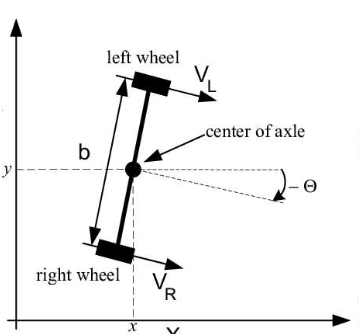
\includegraphics[width = \textwidth]{img/difPod.png}
    \end{minipage}
    \hfill
    \begin{minipage}[b]{0.4\textwidth}
        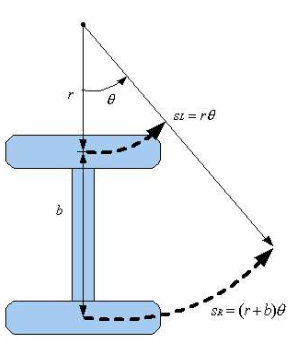
\includegraphics[width = \textwidth]{img/RotCal.png}
    \end{minipage}
\end{figure}

Levý obrázek ukazuje základní pohled na diferenciální podvozek, můžeme na něm vidět hlavní veličiny, které v tomto modelu vystupují, b což je rozteč kol a \(\Theta \) což je úhel natočení od osy.\\
Na pravém obrázků můžeme vidět příklad to jak se počítá cílová vzdálenost, kterou kola urazily, pokud známe úhel o který chceme robota otočit.\\
Pro ovládání robota potřebujeme počítat rychlosti levého a pravého kola, k tomu můžeme potřebovat - průměr kol, počet mikrokroků na jednu otáčku, v případě, že používáme krokový motor k pohonu, při jiných typech motoru potřebujeme otáčky za minutu. \\

\subsection{Matematické řízení}
Rozlišujeme 2 kinematické úlohy, přímou, kterou používáme pro lokalizaci robota a inverzní, kterou používáme pro jeho ovládání.\\
\subsubsection{Přímá úloha kinematiky}
Slouží k měření ujeté vzdálenosti na každém kole a k měření úhlu natočení.\\
Popisuje vztah mezi rychlostí kol a lineární a úhlovou rychlostí podvozku.\\
Následující popis je pro počítání rovnic při užití krokového motoru.\\
\begin{enumerate}
    \item Ujetá vzdálenost levým a pravým kolem během poslední periody vzorkování:
          \begin{center}
              \(\Delta s_L(t) = (\Gamma_L(t)-\Gamma_L(t-t_0))\cdot C_L [m]\)\\
              \(\Delta s_R(t) = (\Gamma_R(t)-\Gamma_R(t-t_0))\cdot C_R [m]\)
          \end{center}
          Konstanty \(C_L\) a \(C_R\) jsou obecně znázorněné parametry kol a motoru(např. vzdálenost ujetá za jeden mikrokrok motoru). \(\Gamma \) je pak počet mikrokroků ujetých za jeden cyklus.
    \item Ujetá vzdálenost celého robota:
          \begin{center}
              \(\Delta s =  \frac{\Delta s_L + \Delta s_R}{2}[m]\)
          \end{center}
    \item Rozdíl úhlu natočení robota mezi posledními okamžiky vzorkování:
          \begin{center}
              \(\Delta \alpha = \frac{\Delta s_L - \Delta s_R}{b}[rad]\)
          \end{center}
          Kde proměnná b je rozteč kol.
    \item Přímá vzdálenost mezi body před a po posledním okamžiku vzorkování:
          \begin{center}
              \(\Delta d = \frac{2\cdot \Delta s}{\Delta \alpha} \cdot \sin(\frac{\Delta \alpha}{2})\)
          \end{center}
    \item Změna souřadnic v souřadnicovém systému:
          \begin{center}
              \(\Delta x(t) = \Delta d(t)\cdot\cos(\alpha(t-t_0)+\frac{\Delta \alpha}{2})\)\\
              \(\Delta y(t) = \Delta d(t)\cdot\sin(\alpha(t-t_0)+\frac{\Delta \alpha}{2})\)\\
          \end{center}
    \item Aktualizace souřadnic podvozku:
          \begin{center}
              \(x(t) = x(t-t_0) + \Delta x(t)\)\\
              \(y(t) = y(t-t_0) + \Delta y(t)\)
          \end{center}
    \item Aktualizace orientace podvozku:
          \begin{center}
              \(\alpha = \alpha(t-t_0) + \Delta \alpha(t)\)
          \end{center}
\end{enumerate}

\subsubsection{Inverzní kinematická úloha}
Řeší ovládání kol robota, pro výpočet rychlosti motorů používáme následující rovnice:\\
\begin{center}
    \(\omega_{L} = (v + 0.5\cdot b \cdot \omega)\cdot \frac{1}{C_L}\)\\
    \(\omega_{R} = (v + 0.5\cdot b \cdot \omega)\cdot \frac{1}{C_R}\)
\end{center}
Kde \(\omega \) je žádaná úhlová rychlost a \(v\) je žádaná rychlost vpřed. Konstanty \(C_L\) a \(C_R\) obecně označují parametry řídicí jednotky pohonu, pohonu, převodovky a kola. Konstanta \(b\) je rozteč kol robota.\\

\subsection{Porovnání s ostatními typy kinematik}
\subsubsection{Diferenciální podvozek}
Výhody diferenciálně řízeného podvozku jsou jeho jednoduchá konstrukce, dobrý manévrovatelnost a možnost zatáčet na místě, bez pohybu vpřed.
Hlavní nevýhodou je jeho neschopnost překonávat vyšší překážky. I velkým robotům s tímto podvozkem dělá problém překonat standardní práh u dveří, což značně limituje možnost prostředí pro jejich využití. \\
\subsubsection{Trojkolový podvozek s řízeným předním kolem}
Tento typ podvozku má hnána 2 zadní kola a přední kolo je motoricky natáčené pro ovládání směru pohybu. \\
Jeho hlavní výhodou je jednoduché ovládání, jedním motorem měníme rychlost pohybu a druhým měníme směr pohybu. Další výhodou je možnost tento podvozek použít terénu narozdíl od podvozku diferenciálního.\\
Nevýhodou oproti diferenciálnímu je však neschopnost se otáčet na místě.\\
\begin{figure}[h!]
    \centering
    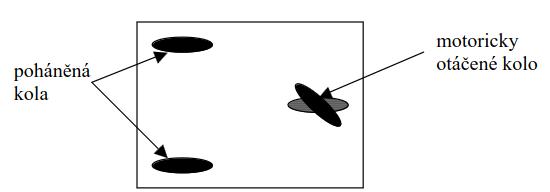
\includegraphics[scale = 0.5]{img/trojkol.png}
\end{figure}
\subsubsection{Podvozky s všesměrovými koly}
Výhoda možnost pohybovat se všemi směry(no shit sherlock), každé kolo obsahuje válečky, díky kterým se robot může hýbat do všech stran. Nevýhodou je složitá konstrukce a je náročnější na kvalitu terénu. Nelze pro něj použít odometrii. \\


\section{Pohony robotů (přehled, vlastnosti, momentové rovnice, požadavky na robotické aplikace, víceosá NC interpolace, rampy, S-křivka).}

\subsection{Přehled druhů motorů}
\subsubsection{Stejnosměrný kartáčový motor}
Jsou nejjednodušší na použití, neboť jsou napájeny pouhým stejnosměrným napájením.\\
Vynikající přetížitelnost. Průměrná možnost měření proudu (zatěžovacího momentu) - mikrozkraty komutátoru, rušení.\\
Sběrače komutátoru - jiskření vede k opotřebení a tudíž nízké životnosti.\\
Kolísání momentu v okamžicích přepínání komutátoru - moment závislý
na poloze rotoru.\\
Je rychlý, je nutno jej zpomalovat mechanickou převodovkou. Vhodný pro rychlostní smyčky(pohon podvozku mobilních robotů).\\
Jednoduché ovládání. \\
\begin{figure}
    \centering
    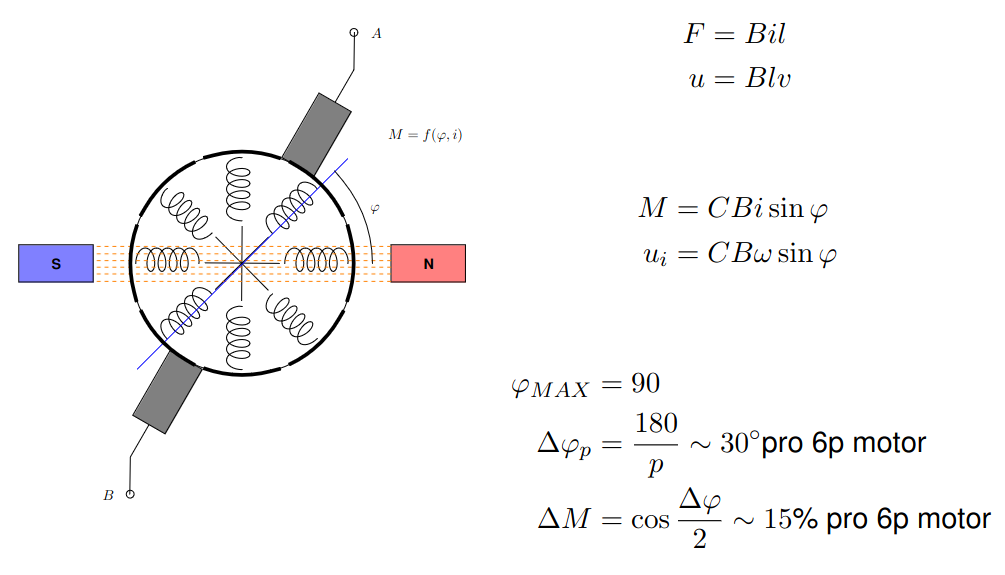
\includegraphics[scale = 0.3]{img/DCMot.png}
\end{figure}
C je konstanta motoru \([N \cdot m \cdot A^{-1}]\)\\

\subsubsection{Stejnosměrný bezkartáčová motor - BLCD}
Bezkartáčový DC motor. Elektronická komutace - menší tření a vyšší otáčky.\\
Stator - 3 cívky, rotor - magnet
Velmi rychlý, taktéž nutno zpomalovat převodovkou.\\
Vhodný pro rychlostní smyčky(pohon vrtulí dronů, pohon mobilních podvozků robotů).\\
\begin{figure}[h!]
    \centering
    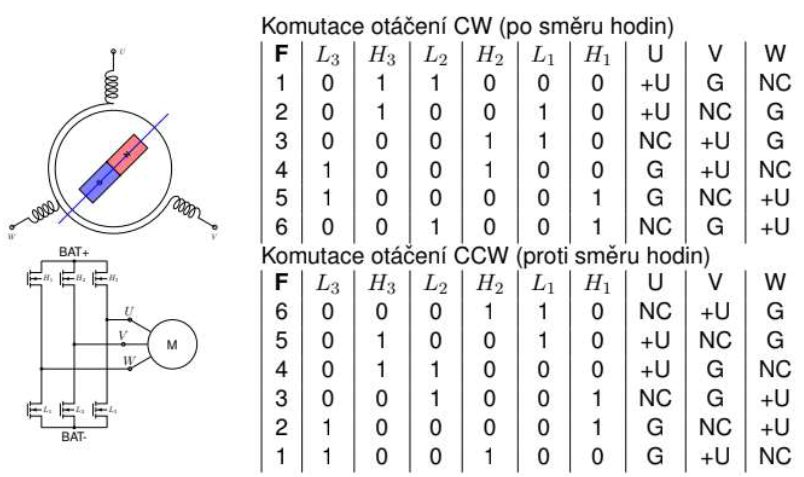
\includegraphics[scale = 0.4]{img/BLCD.png}
\end{figure}

\subsubsection{Krokový motor}
Bezkomutátorový stejnosměrný elektrický motor. Pohyb v krocích, možnost držet rotor v klidu.\\
Rozlišení většinou 200 kroků na otáčku.\\
Je pomalý, vysoká indukčnost L.\\
Energeticky neefektivní, proud teče skrz motor i když není žádný zátěžový moment.\\
Vhodná pro polohové smyčky a NC řízení.\\
Druhy řízení:
\begin{figure}[h!]
    \centering
    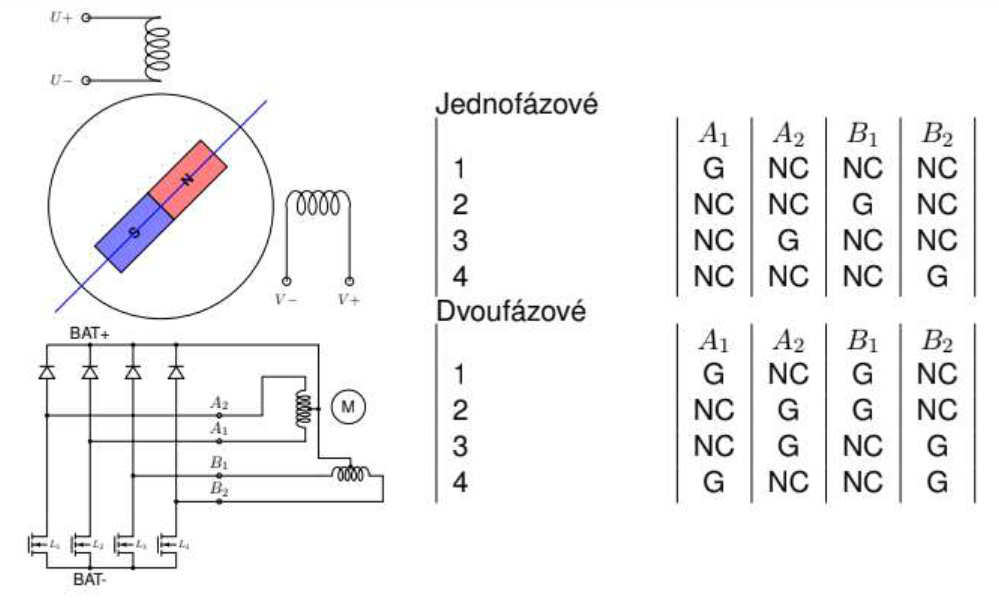
\includegraphics[scale = 0.3]{img/UniPol.png}
\end{figure}
\begin{figure}[h!]
    \centering
    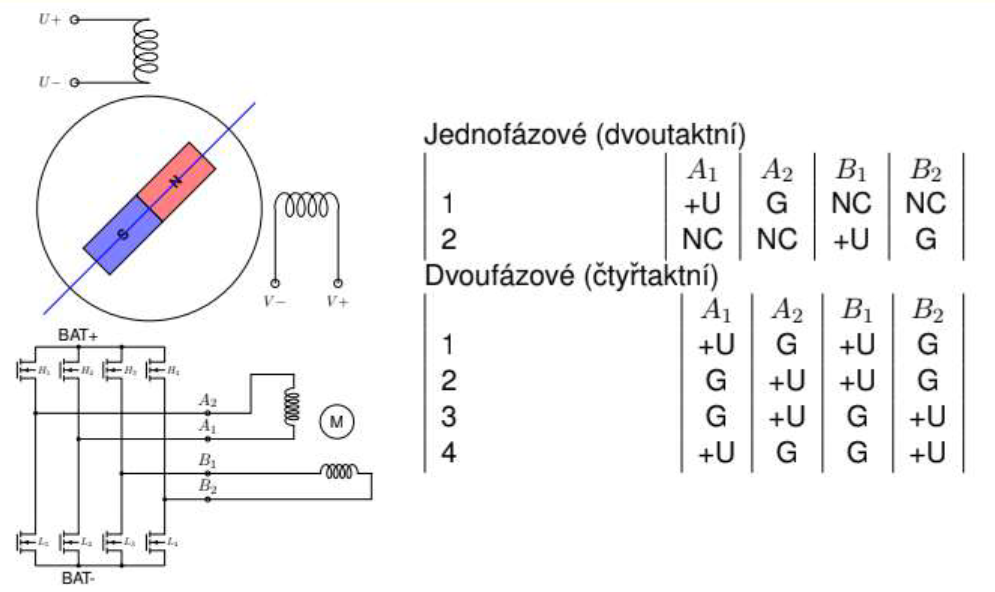
\includegraphics[scale = 0.3]{img/BiPol.png}
\end{figure}

\subsubsection{Synchronní motor PMSM}
Elektronická komutace - menší tření vyšší otáčky. Vynikající možnost měření zatěžovacího momentu.\\
Široký rozsah rychlostí. Energeticky vysoce efektivní.\\
Nízké zvlnění momentu (lze jej řídit v celém rozsahu pozic)\\
Vhodný pro polohové smyčky.\\
\begin{figure}[h!]
    \centering
    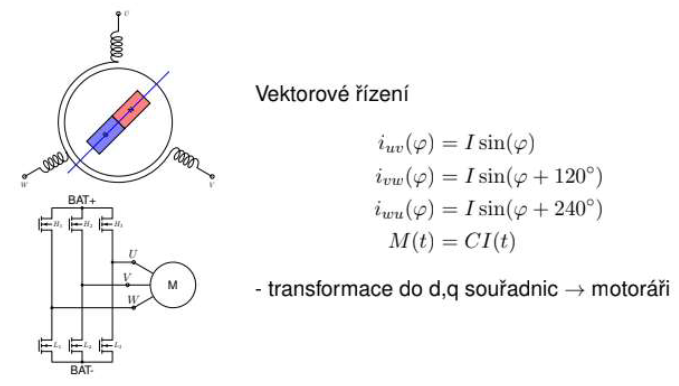
\includegraphics[scale = 0.4]{img/PMSM.png}
\end{figure}
\newpage
\subsection{Momentové rovnice}
\begin{figure}[h!]
    \centering
    \begin{minipage}[b]{0.4\textwidth}
        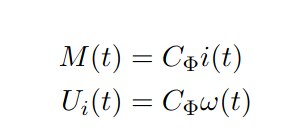
\includegraphics[width = \textwidth]{img/MomRov.png}
    \end{minipage}
    \hfill
    \begin{minipage}[b]{0.4\textwidth}
        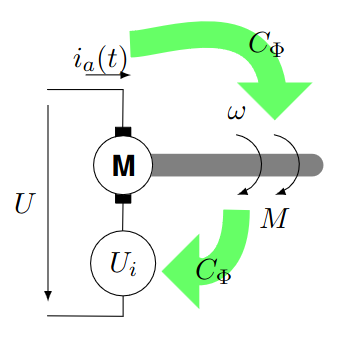
\includegraphics[width = \textwidth]{img/MomRovSchema.png}
    \end{minipage}
\end{figure}
\begin{figure}[h!]
    \centering
    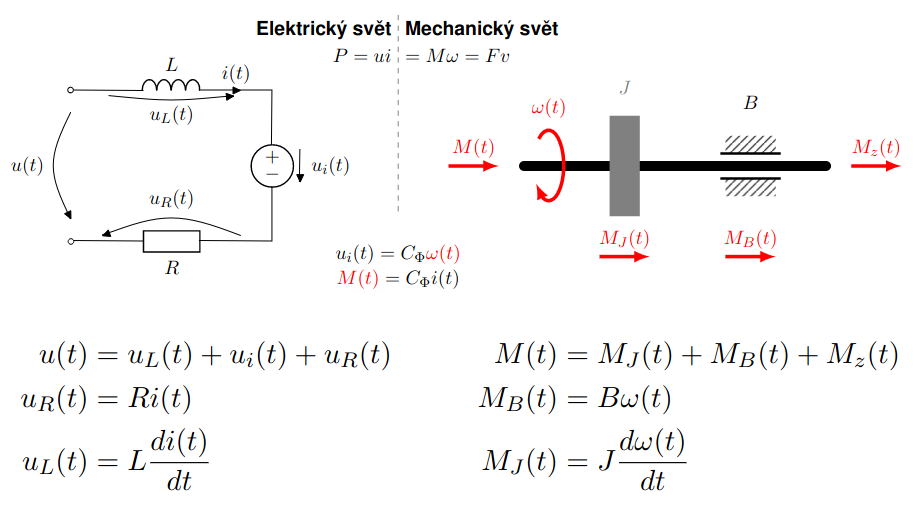
\includegraphics[scale = 0.3]{img/MonRovPrech.png}
\end{figure}
Proměnné v rovnicích:
\begin{itemize}
    \item R - odpor vodiče
    \item L - indukčnost vinutí
    \item \(C_\Phi\) - konstanta motoru
    \item J - setrvačnost
    \item B - tlumení
    \item k - pružnost
    \item \(M_z\) - zatěžovací moment
\end{itemize}
\newpage
\textbf{Za tyhle další se omlouvám protože PRP nemá materiály a internet tyhle pojmy moc nezná}
\subsection{Rampy}
Signál typu rampa pro ovládání motoru znamená graduální zvyšování nebo snižování rychlosti motoru, namísto okamžitého startu či zastavení. Toto zvyšuje životnost motorů, protože na ně není vyvíjen náhlý tlak.
\begin{figure}[h!]
    \centering
    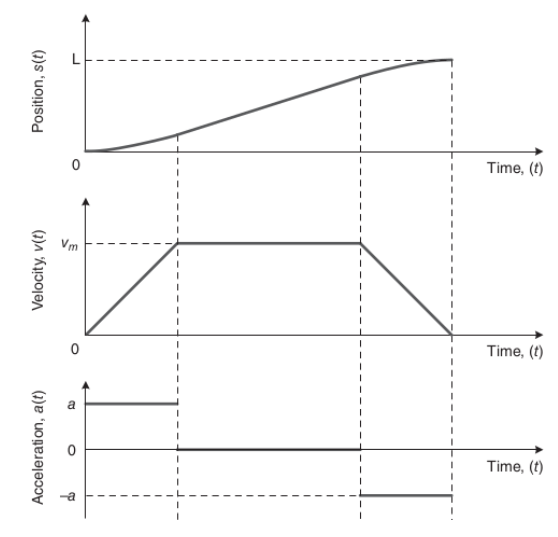
\includegraphics[scale = 0.4]{img/Rampa.png}
\end{figure}
\subsection{S-křivka}
Přesnější rampa, lepší řízení. \\
\begin{figure}[h!]
    \centering
    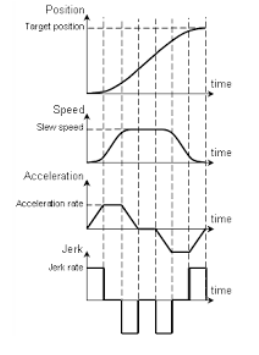
\includegraphics[scale = 0.5]{img/Skrivka.png}
\end{figure}
\subsection{Víceosá NC interpolace}
Interpolace je proces aproximace pohybu po křivce pomocí lineárních úseků.\\
\begin{figure}
    \centering
    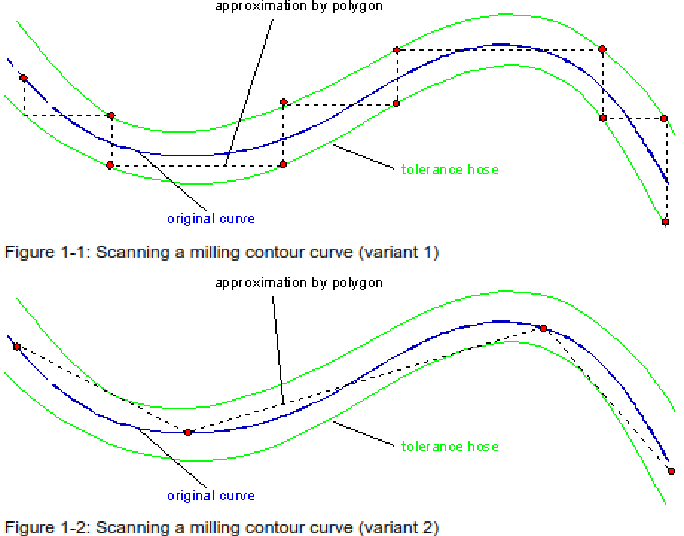
\includegraphics[scale = 0.3]{img/Interolation.png}
\end{figure}

Schéma jedné osy NC interpolátoru:\\
\begin{figure}[h!]
    \centering
    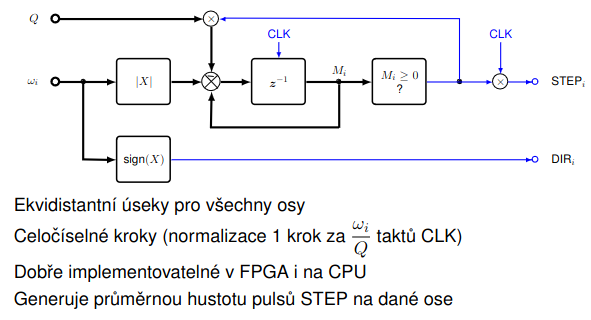
\includegraphics[scale = 0.5]{img/JednaOsaNC.png}
\end{figure}

Průběh NC interpolace:\\
\begin{figure}[h!]
    \centering
    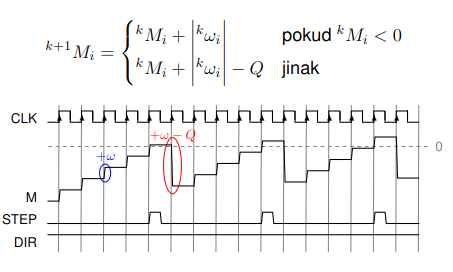
\includegraphics[scale = 0.5]{img/PrubehNCinterpolace.png}
\end{figure}
\section{Systém ROS - popis, platformy, komunikace uvnitř systému, node, message, topic, možnosti reálného nasazení}
\subsection{Popis}
ROS je soubor SW knihoven a nástrojů určených pro vývoj robotických aplikací pracujících na různých platformách, jeho základní částí je knihovna pro síťovou komunikaci, také široké spektrum driverů pro senzory a další software. \\
ROS je middleware, tudíž vytváří interface mezi operačním systémem(podporován je Debian, ale jinak lze i jakýkoliv Linux, avšak bez podpory) a jednotlivými programy.\\
ROS umožňuje komunikaci mezi programem a podprogramy, které mohou být v jiných jazycích, na jiných platformách, či různých počítačích.\\
Jeho součástí je také RVIZ, což je vizualizační program, který umožňuje vytvářet 3D objekty.\\
\begin{figure}[h!]
    \centering
    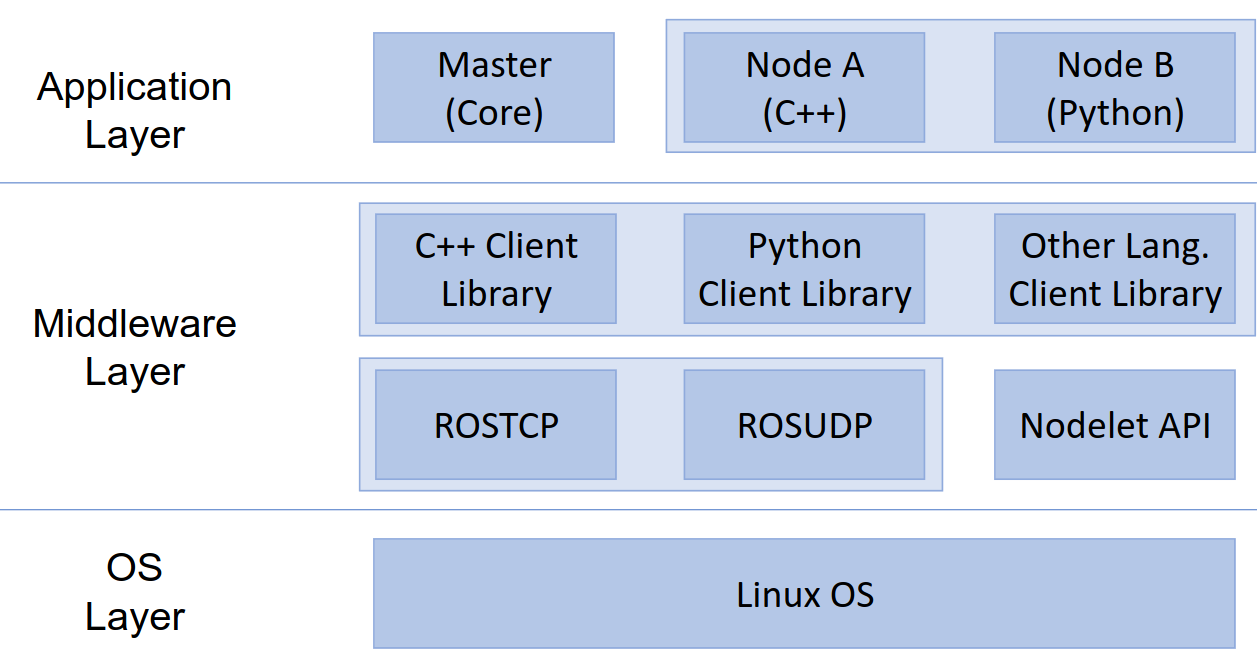
\includegraphics[scale = 0.2]{img/ROSCommMid.png}
\end{figure}
\subsection{Komunikace uvnitř systému}
Master(Core) je komunikační server, který řeší propojení jednotlivých Nodes. \\
Každá node se připojí k masterovi, registrace detailů o topics/messages, které publikuje, service a action, které poskytuje a jaké informace odebírá. Po této registraci master poskytne nodes informace potřebné pro komunikaci mezi nodes.\\
Komunikace mezi Node-Master a Node-Node se provádí pomocí síťového protokolu UDP/TCP.\\
Komunikace mezi jednotlivými Nodes je realizovaná do oddělených kanálů, které nazýváme Topic.
\subsubsection{Publisher-subscriber}
Publisher je instance, která pomocí API publikuje zprávy do určitého topicu. \\
Subscriber příjmá všechny zprávy, které jsou v daném topicku publikované.\\
Každý publisher a subscriber může komunikovat na právě jednom topicu.\\
\begin{figure}[h!]
    \centering
    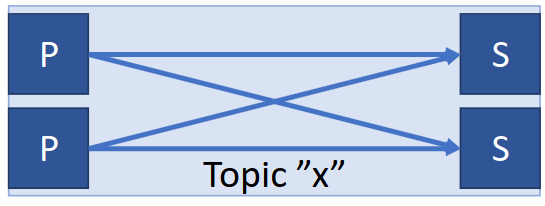
\includegraphics[scale = 0.3]{img/PubSub.png}
\end{figure}
\subsubsection{Server-client}
Jeden node funguje jako server, druhý funguje jako client. Node sloužící jako server čeká na požadavek od klienta a jakmile jej dostane, tak klientovi pošle odpověď.\\
\begin{figure}[h!]
    \centering
    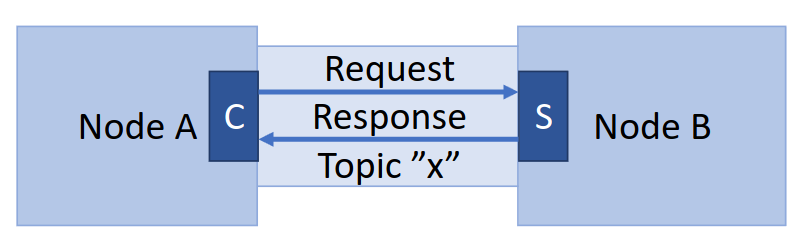
\includegraphics[scale = 0.3]{img/ServClient.png}
\end{figure}
\subsection{Node}
Jeden běžící program využívající ROS client library. Každá node je v ROSu identifikována jménem\\
Individuálně kompilována, spravována, spouštěna. Programovány s využitím ROS knihoven. Pro C++ je to roscpp a pro Python je to rospy.\\
Node by měla být užita pouze pro jeden účel. Například řízení motoru, plánování cesty, preprocessing dat.\\
Nodes mezi sebou mohou komunikovat a měly by komunikovat.\\
Každý node může vytvořit libovolný počet publisherů/subscriberů na libovolné množství topiců.\\
\subsection{Message}
Message je jedna instance předdefinované datové struktury, která bude odeslána z jednoho publishera k N subscriberům.\\
Představuje kontejner pro přenos dat v jednom topicu.\\
\subsection{Topic}
Kanál, který slouží ke komunikaci mezi nodes. Má předdefinované typy dat, které může přenášet.\\
Využívá se k párování publisherů a subscriberů.\\
\begin{figure}[h!]
    \centering
    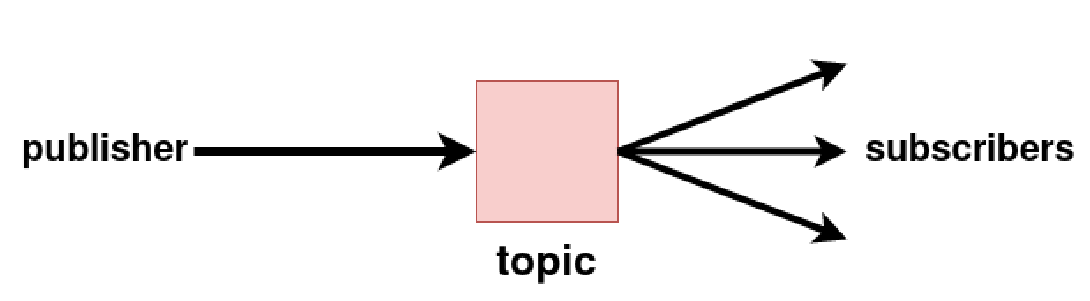
\includegraphics[scale = 0.3]{img/Topic.png}
\end{figure}

\subsection{Možnosti reálného využití}
Pro simulaci robota, pomocí RVIZ.\\
Kontrola více dronů:
\begin{figure}[h!
    ]
    \centering
    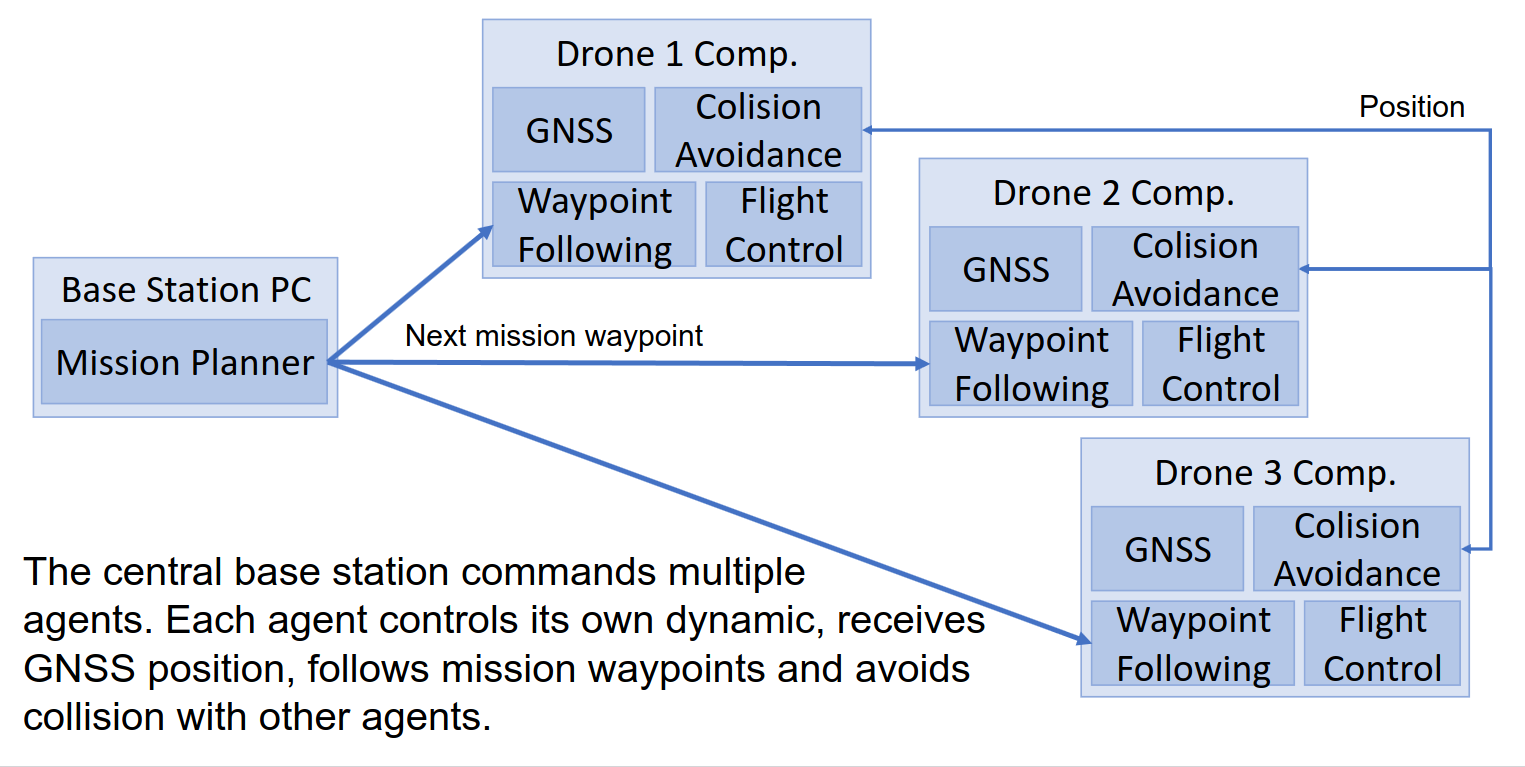
\includegraphics[scale = 0.3]{img/ROSControl.png}
\end{figure}
\section{Zpětnovazební regulace pozice mobilního robotu při sledování trajektorie (nákres, regulační schéma, popis veličin v procesu, popis parazitních vlivů ovlivňujících kvalitu regulace v důsledku implementace do reálného stroje).}

\subsection{Nákres a regulační schéma}
Toto schéma platí pro použití diferenčního podvozku, kde regulujeme úhlovou a lineární rychlost, nastavujeme dva motory, které ženou kola a zpětná vazba je tvořena snímačem na robotovi.

\begin{figure}[h!]
    \centering
    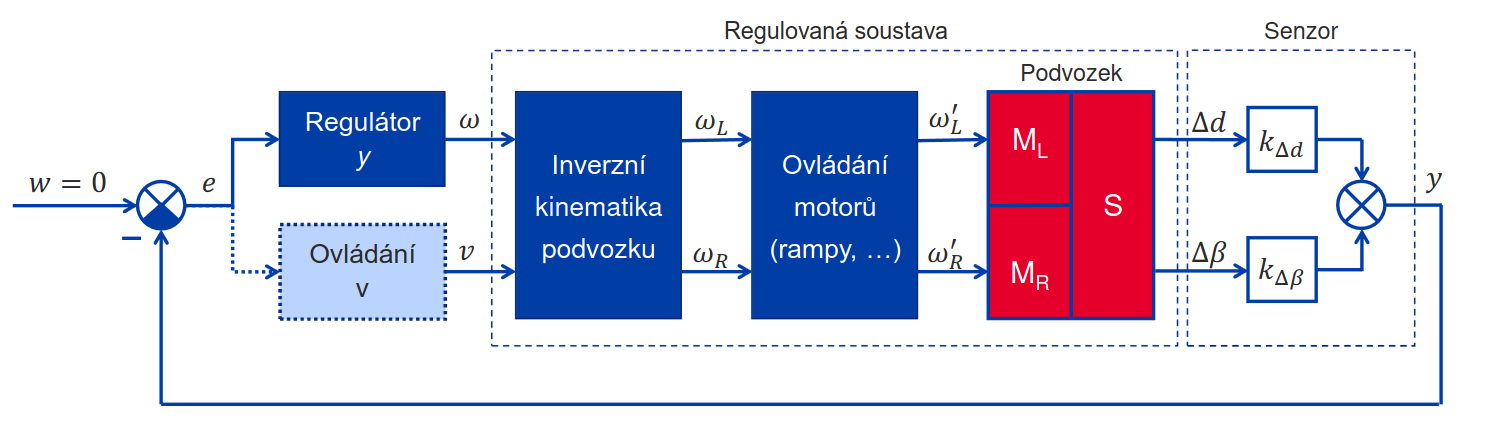
\includegraphics[scale = 0.3]{img/RegSoust.png}
\end{figure}
Kde w je žádaná hodnota, v našem případě je to odchylka od čáry, která je samozřejmě 0. y je výstupní hodnota reprezentující polohu robota vůči čáře. \(\omega \) a v jsou výstupy vstupy do inverzní kinematické úlohy podvozku, ze které dostaneme úhlové rychlosti pro jednotlivá kola \(\omega_R\) a \(\omega_L\). Poté jsou pomocí části programu pro ovládání motoru transformovány na \(\omega_{L}^{'}\) a \(\omega_{R}^{'}\). Veličinami vystupujícími ze samotného robota, které jsou získány pomocí přímé úlohy kinematiky pak jsou \(\Delta d\) a \(\Delta \beta \).\\

Poruchové veličiny mohou vstupovat v různých místech, nejvýznamnější poruchou v našem případě je odchýlení čáry od aktuální trajektorie robota.\\

\subsection{Parazitní vlivy}
\subsubsection{Snímání čáry}
\begin{enumerate}
    \item Všechny parazitní vlivy týkající se optočlenů
    \item Přesnost kalibrace, musíme vědět jaká je v prostředí maximální a minimální hodnota vycházející z optočlenů, potažmo A/D převodníku. Tyto krajní hodnoty v realitě odpovídají plnému najetí a vyjetí z trajektorie.
\end{enumerate}

\subsubsection{Pohon}
\begin{enumerate}
    \item Mechanické vůle, nepřesnosti
    \item Přesnost kalibrace - rozměry kol, rozteč kol, výpočet konstant pro podvozek
    \item Prokluz kol
    \item Přesnost mikrokrokování
\end{enumerate}

\subsubsection{Obecné}
\begin{enumerate}
    \item Zpoždění kvůli komunikaci - variabilní zpoždění regulační smyčky podle délky komunikace
    \item Neúspěchy při komunikaci - výpadek
    \item Výpočetní výkon
    \item Neoptimalizovaný SW
    \item Špatné odladění PSD regulátoru, špatné potlačení wind-up jevu
\end{enumerate}
